\documentclass[11pt]{article}

\usepackage[margin=1in]{geometry}
\usepackage[utf8]{inputenc}
\usepackage[T1]{fontenc}
\usepackage{times}
\usepackage{microtype}
\usepackage{amsmath,amssymb,amsthm}
\usepackage{booktabs}
\usepackage{multirow}
\usepackage{graphicx}
\usepackage{xcolor}
\usepackage[numbers,sort&compress]{natbib}
\usepackage{algorithm}
\usepackage{algpseudocode}
\usepackage[colorlinks=true,linkcolor=blue!60!black,citecolor=blue!60!black,urlcolor=blue!60!black]{hyperref}
\usepackage[capitalize,noabbrev]{cleveref}

\newtheorem{proposition}{Proposition}
\newcommand{\R}{\mathbb{R}}
\newcommand{\E}{\mathbb{E}}
\DeclareMathOperator{\Diag}{diag}

\title{\textbf{A Counterexample to the Forgetting Waterbed}}
\author{AI-generated by Devin (Cognition AI)}
\date{}
\hypersetup{pdftitle={A Counterexample to the Forgetting Waterbed},pdfauthor={AI-generated by Devin (Cognition AI)}}

\begin{document}
\maketitle

\begin{abstract}
Continual learners trade retention against adaptation as the mix of old and new tasks changes.
A proposed waterbed law makes this tradeoff spectral: reducing the response of old-task loss at one switching frequency should increase it elsewhere if final accuracy is matched.
We test this claim by driving the task mixture of a two-layer linear learner at 55 frequencies across eight paired seeds, comparing two gradient-descent rates, replay, and elastic weight consolidation in a 12-second CPU sweep.
A linearized transfer predicts the measured mean log-gains within 0.0065 log units, yet the raw areas vary by 46.3\% across methods, exceeding the 20\% rejection threshold despite matched terminal joint accuracy.
Changing only the learning rate raises old-task loss gain at every sampled frequency without changing the unforced fit.
Jensen's formula explains why: the area depends on the first nonzero impulse coefficient and any zeros outside the unit circle, and dividing by the one-step gain removes the area difference to within 0.0065 log units in this minimum-phase rig.
\end{abstract}

\section{Introduction}
\label{sec:intro}

Continual learning methods limit forgetting by reusing old examples or restricting how far parameters move from a previous solution~\citep{rolnick2018,kirkpatrick2016}. Their retention depends on the stream: an old task may return after one update or after a long run on another task. A frequency-domain view asks whether tuning for one timescale necessarily hurts another. If the total log-gain were fixed at a matched final fit, a retention method could move sensitivity across frequencies but could not lower it throughout the spectrum.

We test this prediction by modulating the old-task fraction around a fixed mixture. In \cref{fig:spectra}, increasing only the learning rate increases the old-task loss response at every sampled frequency. No compensating reduction appears. A lock-in calibration with known harmonics and a separate linearized transfer recover the expected responses (\cref{sec:calibration}); the discrepancy is with the invariance claim, not with the estimator.

Different terminal fits could explain gain differences between replay and consolidation. The two gradient-descent arms remove that explanation: they use the same teachers and initialization, take the same number of steps, and reach the same unforced predictor, with identical per-task losses. The rate change alone produces a 1.782 log-unit area gap. Across all four arms, the range is 46.3\% of the mean absolute area, beyond the specified 20\% rejection threshold (\cref{tab:main,tab:ablations}).

The distinction is between a closed-loop sensitivity with a fixed leading coefficient and an input-to-loss transfer whose leading coefficient can change. The one-step loss response depends on the learning rate, the operating point, and how the update uses the incoming mix. We identify that coefficient and the out-of-circle zeros as the relevant terms (\cref{prop:jensen}). The resulting conditional identity describes the local response; it does not constrain absolute forgetting or guarantee a tradeoff in stochastic training.

\begin{figure}[!t]
  \centering
  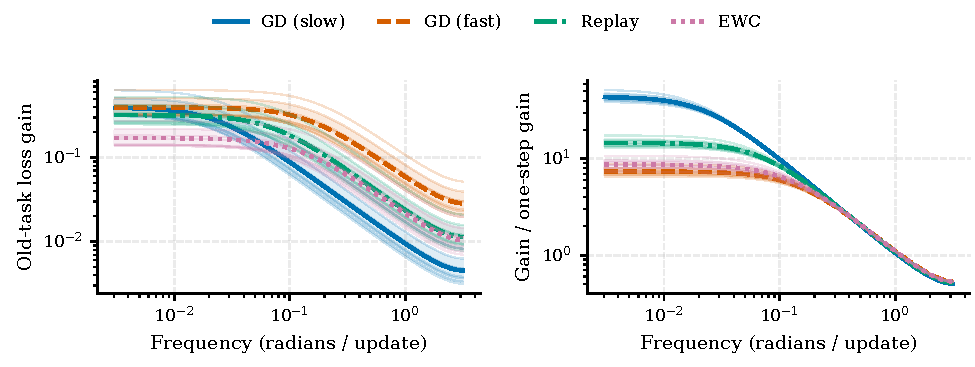
\includegraphics[width=\textwidth]{spectra.pdf}
  \caption{\textbf{The learning-rate change raises raw gain throughout the sampled band.}
  Left: gain from old-task fraction to old-task squared loss at amplitude 0.01 over 55 frequencies up to Nyquist. Right: gain divided by the absolute one-step gain for each arm and seed. Heavy lines are geometric means across eight paired seeds; bands are pointwise 95\% Student-\(t\) intervals on log-gain; faint lines are individual seeds. GD is gradient descent; EWC is elastic weight consolidation.}
  \label{fig:spectra}
\end{figure}

\section{Problem statement}
\label{sec:problem}

Let \(A\) be an old task initially solved by the learner, and \(B\) a conflicting new task. At step \(t\), let \(u_t\in[0,1]\) denote the incoming old-task fraction.

The learner scores its current parameters on \(A\), then updates using the mixture and any method-specific memory. We drive \(u_t=\tfrac12+\alpha\cos(\omega t)\), with amplitude \(\alpha>0\) and frequency \(\omega\) in radians per update. The old-task loss is \(\ell_A(\theta_t)\), where \(\theta_t\) denotes the parameters before update \(t\). The transfer \(S\) maps a small perturbation of \(u_t\) to a perturbation of this loss at the unforced operating point. The measured gain is the fundamental harmonic amplitude of the settled loss divided by \(\alpha\).

We test the mean log-area
\begin{equation}
  \mathcal{I}=\frac{1}{\pi}\int_0^\pi \log |S(e^{i\omega})|\,d\omega.
  \label{eq:area}
\end{equation}
The raw claim predicts that the range of \(\mathcal I\) is at most 20\% of its mean absolute value at matched terminal joint accuracy. This threshold is a decision rule in fixed loss units, not a scale-invariant physical constant: multiplying the loss by a common factor shifts each area by the same log constant. We therefore report the area difference and its exponential, the ratio of geometric-mean gains. The area weights frequencies uniformly in \(\omega\), not uniformly on the logarithmic axis used to draw \cref{fig:spectra}.

The output is loss, not classification accuracy: at a point where the gradient of old-task loss vanishes, the first-order loss transfer vanishes even if the predictor moves. We measure retention separately as terminal sign accuracy and the mean increase in old-task loss from the initial fit. This separates steady operating-point degradation from the response to a small change in the mix. Cyclic forgetting bounds and tracking analyses answer different questions: they bound a loss after repeated task exposures or track a moving optimum, rather than integrating the old-task loss response around a fixed mixture.

\section{A mixer-to-loss experiment}
\label{sec:method}

\subsection{Two teachers and one learner}

Both tasks use \(x\sim\mathcal N(0,\Sigma)\), with a positive diagonal covariance \(\Sigma\in\R^{d\times d}\) and \(d=4\). The teachers have slopes \(a,b\in\R^d\) and clean labels \(x^\top a,x^\top b\), respectively. Both teacher outputs have unit variance; their angle in whitened coordinates lies between 0.80 and 1.20 radians. The width-one two-layer student predicts \(v w^\top x\), with \(w\in\R^d\) and \(v\in\R\). Both factors in \(\theta=(w,v)\in\R^{d+1}\) are trained. Writing \(\beta=vw\), its population losses are
\begin{equation}
  \ell_A(\theta)=\tfrac12(\beta-a)^\top\Sigma(\beta-a),\qquad
  \ell_B(\theta)=\tfrac12(\beta-b)^\top\Sigma(\beta-b).
  \label{eq:loss}
\end{equation}
Every arm starts at the same balanced factorization \(\theta_A\) of \(\beta=a\), where \(v>0\) and \(\|w\|_2=v\). The stream is an intervention on the mixture of two population gradients. It is not a stream of noisy minibatches: this removes gradient noise and fixes a well-defined operating point for the transfer.

Let \(r\) be the replay fraction and \(\lambda\) the consolidation strength. All four arms use a single gradient-descent update with rate \(\eta\):
\begin{align}
  \theta_{t+1}&=\theta_t-\eta\nabla_\theta J(\theta_t,u_t), \label{eq:update}\\
  J(\theta,u)&=(1-r)\{u\ell_A(\theta)+(1-u)\ell_B(\theta)\}
    +r\widehat\ell_A(\theta)
    +\tfrac{\lambda}{2}(\theta-\theta_A)^\top D(\theta-\theta_A). \label{eq:objective}
\end{align}
Here \(\widehat\ell_A\) is squared loss on 512 cached examples labeled by \(A\). Its gradient depends on the cache only through the empirical input covariance. The diagonal matrix \(D\in\R^{(d+1)\times(d+1)}\) contains the population second moments of the per-example squared-loss gradients at \(\theta_A\), under a Gaussian label-noise variance of \(0.0625\). This is the Gaussian model's diagonal Fisher rescaled to the squared-loss convention. The noise defines this penalty only; both the stream and the evaluation use clean targets. Gradient descent sets \(r=\lambda=0\); replay sets \(r=0.10,\lambda=0\); elastic weight consolidation (EWC) sets \(r=0,\lambda=8\).

\subsection{Settled response rather than transient forgetting}

We first warm up each arm at \(u_t=1/2\). Each driven run starts from that arm's unforced parameters \(\theta_\star\). We score \(\ell_A(\theta_t)\) before applying update \(t\), discard the first 2,048 driven steps, and fit cosine and sine coefficients over the next 8,192 steps. We snap a logarithmic grid to integer Fourier bins. A constant offset is orthogonal to both fitted harmonics; at Nyquist we fit only cosine and use its full squared norm. We divide the resulting magnitude by \(\alpha\) and integrate a shape-preserving cubic interpolant of log-gain. The first bin is at \(0.00307\) radians per update; we extend the log-gain flat from that bin to zero and also compute the area without this extension.

Why use a mixture rather than hard switches? A small drive separates the local response from the large moves induced by a new task. It also gives a direct diagnostic: doubling \(\alpha\) should leave the gain approximately unchanged if higher-order effects are small. In contrast, the old-task loss mean need not decrease when the gain decreases. We report both and do not use either as a proxy for the other.

\subsection{What the log-area depends on}

Write \(p=d+1\). Linearize \cref{eq:update} at \((\theta_\star,\tfrac12)\), and read out the perturbation in \(\ell_A\). With state \(s_t=\theta_t-\theta_\star\), input \(\delta u_t=u_t-\tfrac12\), and scalar output perturbation \(\delta y_t\), the first-order system is
\begin{align}
  s_{t+1}&=M s_t+g\,\delta u_t,\qquad \delta y_t=c^\top s_t,\label{eq:lti}\\
  M&=I_p-\eta\nabla_\theta^2 J,\quad
  g=-\eta\,\partial_u\nabla_\theta J,\quad c=\nabla_\theta\ell_A.
\end{align}
Here \(M,I_p\in\R^{p\times p}\) and \(g,c\in\R^p\); derivatives are evaluated at the unforced point. The transfer \(S(z)=c^\top(zI_p-M)^{-1}g\) is strictly proper because we score before updating. Its one-step coefficient is \(h_1=c^\top g\). The two-layer scaling direction can be neutral without appearing in \(S\); only poles of the scalar transfer enter the calculation. In particular, a hidden neutral mode does not justify assuming stability if the readout sees it.

\begin{proposition}[Log-area of the local transfer]
\label{prop:jensen}
Let \(S\) be a nonzero real rational transfer with all poles strictly inside the unit circle. Let \(h_m\) be its first nonzero impulse coefficient, \(m\geq 1\), and let \(\zeta_k\) be its finite zeros, counted with multiplicity. Then
\begin{equation}
  \mathcal I=\log|h_m|+\sum_{k:\,|\zeta_k|>1}\log|\zeta_k|,
  \label{eq:jensen}
\end{equation}
\end{proposition}

The rational factorization of \(S\) has leading numerator-to-denominator coefficient \(h_m\). On the unit circle, the log integral of each factor \(z-q\) is \(\log\max(1,|q|)\), by Jensen's formula. Stable poles contribute zero; because the coefficients are real, the average over positive frequencies equals the full-circle average. \Cref{app:proof} gives the details and a nonminimum-phase example.

Thus \(h_1\neq 0\) and minimum phase imply zero normalized area after dividing the gain by \(|h_1|\), not equal raw area. Equal raw areas require the right-hand side of \cref{eq:jensen} to stay fixed, which matching prediction accuracy does not enforce. Even the normalized equality constrains the integral, not pointwise gains or mean retention.

\section{Experimental setup and results}
\label{sec:results}

\subsection{Paired sweep and budgets}

Each of the eight seeds defines one teacher pair, input covariance, and replay cache, shared by all arms. We use 8,192 unforced warm-up steps per arm and seed, then 10,240 driven steps for each of 55 frequencies and two amplitudes. Every arm trains five parameters. Replay stores a dense \(4\times4\) Gram matrix of the old examples (128 bytes in float64); EWC retains the five anchor parameters and five Fisher weights (80 bytes). These are auxiliary algorithmic state sizes, not total program memory. Teacher parameters and the validation readout are part of the simulator, not counted as extra memory for one method. Replay adds a covariance-vector product, EWC adds a diagonal penalty gradient, and the two gradient-descent arms have identical update arithmetic. We do not claim FLOP parity across the memory arms or an implementation speedup.

The sweep took 12.14 CPU seconds and 12.17 wall seconds on an x86-64 CPU VM, with one OpenBLAS thread. The measurement starts from freshly copied warm-up states; neither scoring nor future mixture values enter a learner update. Population accuracy is computed analytically on independent draws from the input distribution rather than on the replay cache. Intervals are Student-\(t\) intervals over seeds; the learning-rate contrast is paired. Frequencies and time steps are not replicates. The seed generator and all run settings are in \cref{app:details}.

\subsection{Estimator controls}
\label{sec:calibration}

The lock-in recovers injected first harmonics at an interior Fourier bin and at Nyquist. For independent minimum- and nonminimum-phase rational filters, dense numerical integration and the root formula agree with their known areas to \(10^{-12}\) in the self-test (\cref{app:proof}). For the fitted transfers in the actual sweep, dense LTI integration agrees with \cref{eq:jensen} to \(9\times 10^{-16}\) log units; applying the finite experimental grid to the LTI response changes the area by at most \(3.3\times10^{-5}\). These checks distinguish numerical integration and harmonic normalization from the behavior of the trained learner.

The larger amplitude changes fitted gain by at most 3.89\% across all arms, seeds and frequencies; the maximum occurs at Nyquist for fast gradient descent. At the primary amplitude 0.01, measured gain is within 1.37\% of the linear prediction at every sampled point, and measured area is within 0.0065 log units of the exact transfer integral. The measured gains are therefore close to, but not identical to, the infinitesimal response.

\subsection{The raw area is not conserved}

\begin{table}[!t]
  \centering
  \small
  \setlength{\tabcolsep}{4pt}
  \caption{\textbf{Matched joint accuracy does not yield matched log-area.}
  Means at amplitude 0.01 across eight paired seeds; uncertainty on measured area is a 95\% seed-level interval half-width. Final \(A\) accuracy and mean \(A\) loss also average over 55 frequencies. The Jensen column is computed from the linearization, not fitted to the measured gain. Auxiliary bytes exclude the five common trainable parameters and simulator state.}
  \label{tab:main}
  \begin{tabular}{lrrrrr}
    \toprule
    Method & Measured area & Jensen area & Mean \(A\) loss \(\downarrow\) & Final \(A\) acc. \(\uparrow\) & Aux. bytes \\
    \midrule
    GD, slow & \(-4.716\pm0.277\) & \(-4.716\) & 0.10137 & 85.31\% & \textbf{0} \\
    GD, fast & \(-2.934\pm0.274\) & \(-2.931\) & 0.10138 & 85.39\% & \textbf{0} \\
    Replay & \(-3.824\pm0.282\) & \(-3.823\) & 0.08262 & 86.91\% & 128 \\
    EWC & \(-3.931\pm0.290\) & \(-3.931\) & \textbf{0.04462} & \textbf{90.72\%} & 80 \\
    \bottomrule
  \end{tabular}
\end{table}

Terminal joint accuracy averages the two teachers' sign accuracies. It is about 85.22\% for each arm in \cref{tab:main}; the largest cross-method gap over all paired endpoints is 0.00082 percentage points, below the 1-point matching tolerance. This metric is insensitive to shifting fit toward one teacher: for a student direction on the arc between the two whitened teachers, the two angular errors sum to the teacher angle. Consequently, we do not treat this match as a match of individual task scores. EWC's lower old-task loss comes with worse new-task fit (unforced losses in \cref{tab:unforced}).

The raw area range is 46.26\% of the across-method mean absolute area. The implied geometric-mean gain ratio is 5.94, and mean old-task loss differs by a factor of 2.27. In the two gradient-descent arms alone the spread is 46.58\%; the paired area contrast is \(1.782\) log units (95\% CI \([1.779,1.785]\)). Their unforced predictions and both per-task losses match, so a different terminal fit is not needed to obtain a different area. The fast arm's gain exceeds the slow arm's at all sampled frequencies and seeds (\cref{fig:spectra}): the smallest fast-to-slow ratio is 1.007.

\subsection{What changes the area?}

\begin{table}[!t]
  \centering
  \small
  \caption{\textbf{Rate changes the area more than drive amplitude does.}
  The base is fast gradient descent. Blank settings retain the base value. Rows change one factor, with the same eight paired seeds and update counts. Areas are seed means; the main rate contrast has a paired 95\% interval \([1.779,1.785]\) for fast minus slow.}
  \label{tab:ablations}
  \begin{tabular}{llrrrr}
    \toprule
    & Variant & Rate \(\eta\) & Drive \(\alpha\) & Raw area & Gain-normalized area \\
    \midrule
    & \texttt{base} & 0.150 & 0.01 & \(-2.9345\) & \(-0.0034\)\\
    \midrule
    (A) & Slower update & 0.025 & & \(-4.7162\) & \(-0.0001\)\\
    (B) & Larger drive & & 0.02 & \(-2.9447\) & \(-0.0136\)\\
    \bottomrule
  \end{tabular}
\end{table}

\textbf{(A) Is the leading gain the missing quantity?}
The fast and slow arms share the operating predictor, but the mean absolute one-step gain changes from 0.00942 to 0.05609. All fitted zeros are inside the unit circle (largest modulus 0.9851). Subtracting the log absolute one-step gain removes most of the observed area difference (\cref{tab:ablations}). Across all four arms, the largest normalized area range within a seed is 0.00644 log units. The normalized spectra themselves differ, as \cref{fig:spectra} shows.

\textbf{(B) Does finite drive explain the failure?}
Doubling the drive changes the fast arm's mean area by 0.0102 log units, compared with the 1.782-log-unit rate contrast at the base amplitude. The finite-amplitude area is slightly biased relative to the LTI calculation, most visibly for fast gradient descent, but the discrepancy is too small to explain the rate effect. Omitting the near-DC flat extension leaves every method's mean log-area within 0.004 log units of its primary estimate.

\paragraph{An exact scalar check.}
The result does not require two-layer scale dynamics. For a one-parameter regressor with unit input variance and unit-separated teachers, the mixed optimum is \(1/2\) after choosing slopes 0 and 1. For rate \(0<\eta<1\), its loss transfer is \(S(z)=(-\eta/2)/(z-(1-\eta))\), and its log-area is \(\log(\eta/2)\). At every nonzero frequency the magnitude strictly increases with \(\eta\); at DC it is the same for both rates (\cref{app:proof}). This exact alternate model tests the directional finding without interpolation, cache noise, or an internal scaling direction. It is not a replication on nonlinear or stochastic learners.

\section{Related work}

\paragraph{Forgetting under repeated exposure.}
Linear-regression analyses relate forgetting to task ordering, learning rate, and the geometry of sequential projection~\citep{ding2024,cyclic2023}. In cyclic document training, old examples can recover before their next presentation~\citep{yang2024}. These studies motivate measuring timescales, but analyze loss after task exposures or trajectories under hard recurrence; we instead estimate an infinitesimal response around a stationary mixture.

\paragraph{Control and frequency-domain probes.}
Discrete-time Bode and complementary-sensitivity theory already give the integral and its dependence on leading coefficients and nonminimum-phase zeros~\citep{emami2019,wan2018}. Frequency-domain analyses of online optimization characterize tracking of moving optima~\citep{vanscoy2025}; control minimization uses dynamics to protect learned representations~\citep{dehaan2026}. Sinusoidal probing has also been used to characterize reasoning sensitivity to prompt parameters~\citep{wang2025}. Our contribution is neither a new control identity nor a new retention method: it is a counterexample for the old-task loss readout and a diagnostic for when its normalized area is constrained.

\section{Conclusion}

At the same unforced fits and update count, changing only the learning rate raises the old-task loss gain throughout the sampled band. The raw area misses the invariance criterion (\cref{tab:main,tab:ablations}). Its local prediction instead depends on the first impulse coefficient and the out-of-circle zeros. Only after removing that coefficient do the minimum-phase areas agree (\cref{prop:jensen,fig:spectra}).

This test uses two conflicting linear teachers, exact gradients, and a small sinusoidal drive. It does not establish an invariant for changing operating points, finite-sample training, or nonminimum-phase transfers. Matching joint accuracy also does not match every old and new score. The \href{https://github.com/manojbajaj95/cl/tree/f018cf8/experiments/waterbed}{experiment, seed-level data, and estimator checks} are available for reproduction; the next empirical test is whether a stable local transfer is informative under noisy minibatch streams.


\bibliographystyle{plainnat}
\bibliography{references}

\appendix
\section{Transfer derivations and estimator controls}
\label{app:proof}

\paragraph{Log integral.}
Cancel common roots and write \(S(z)=h_m\prod_k(z-\zeta_k)/\prod_j(z-\rho_j)\), where \(\rho_j\) are the finite poles and the denominator degree exceeds the numerator degree by \(m\). The expansion at infinity starts at \(h_m z^{-m}\), which fixes the coefficient in this factorization. For \(|q|<1\), \(\log|e^{i\omega}-q|=\operatorname{Re}\log(1-q e^{-i\omega})\), whose Fourier expansion has zero average. For \(|q|>1\), factor out \(-q\) first to obtain mean \(\log|q|\). For \(|q|=1\) the logarithmic singularity is integrable and the average is zero by the limiting formula. Apply this identity to each factor and use conjugate symmetry to recover \cref{eq:jensen}.

\paragraph{Exact scalar contrast.}
For teacher slopes 0 and 1, write the learner coefficient as \(\beta_t\). The update is \(\beta_{t+1}=(1-\eta)\beta_t+\eta(1-u_t)\), and the old loss is \(\tfrac12\beta_t^2\). Thus at \(\beta_\star=\tfrac12\), \(g=-\eta\) and \(c=\tfrac12\). The squared gain is
\[
  |S(e^{i\omega})|^2 =
  \frac{1}{4}\left[1+\frac{2(1-\eta)}{\eta^2}(1-\cos\omega)\right]^{-1}.
\]
The factor \((1-\eta)/\eta^2\) strictly decreases for \(0<\eta<1\). This proves the strict ordering for \(0<\omega\leq\pi\) even though both arms have identical DC gains, \(\lvert S(1)\rvert=\tfrac12\).

\paragraph{Nonminimum-phase boundary.}
The estimator checks use \(0.2/(z-0.8)\), with area \(\log 0.2\), and
\[
  -\frac{6}{z-0.2}+\frac{7}{z-0.5}
    =\frac{z+1.6}{(z-0.2)(z-0.5)},
\]
with area \(\log 1.6\). The latter has two stable poles and unit one-step gain, but its zero at \(-1.6\) gives positive normalized area. It is an analytic filter control, not a transfer fitted to another continual learner. The lock-in control injects a nonzero offset plus known cosine and sine coefficients at a Fourier bin and verifies the Nyquist cosine-only normalization separately.

\paragraph{Fitted transfer calculation.}
For the product \(\beta=vw\), the Jacobian is \(P=[vI_d\;\;w]\in\R^{d\times p}\). Let \(\widehat\Sigma_A\) denote the cache covariance, and \(q\in\R^d\) the gradient of the data terms of \(J\) with respect to \(\beta\) at the unforced point. The parameter Hessian is \(P^\top[(1-r)\Sigma+r\widehat\Sigma_A]P+\lambda D\) plus a symmetric block with \(q\) and \(q^\top\) in the cross derivatives between \(w\) and \(v\). At a stationary point with \(r>0,\lambda=0\), or with \(r=\lambda=0\), \(q=0\) for nonzero \(v\); EWC can have \(q\neq0\). Input and readout vectors are \(g=-\eta(1-r)P^\top\Sigma(b-a)\) and \(c=P^\top\Sigma(\beta-a)\). Diagonalizing the symmetric \(M\) gives each residue as the product of \(g\) and \(c\) projected onto that mode. The implementation drops residues below \(10^{-12}\) of the maximum magnitude, rejecting unstable retained poles, and asserts stationarity at absolute tolerance \(10^{-8}\).

\section{Reproduction details}
\label{app:details}

For each NumPy seed 410--417, draw the diagonal entries of \(\Sigma\) uniformly from \([0.65,1.35]\). Take orthonormal columns \(e_1,e_2\in\R^d\) from the QR factorization of a \(d\times2\) standard Gaussian matrix; set \(a=\Sigma^{-1/2}e_1\) and \(b=\Sigma^{-1/2}(\cos\gamma\,e_1+\sin\gamma\,e_2)\) for \(\gamma\) uniform on \([0.8,1.2]\). Cache vectors are independent draws from \(\mathcal{N}(0,\Sigma)\). The prior anchor has \(v=\sqrt{\|a\|_2}\) and \(w=a/v\). Joint sign accuracy follows from Gaussian angular agreement, \(1-\varphi/\pi\) for the angle \(\varphi\) between \(\Sigma^{1/2}\beta\) and the corresponding whitened teacher. No test samples or labels enter the simulator updates.

\begin{table}[htbp]
  \centering
  \caption{\textbf{Joint sign accuracy can hide a shift from the new teacher to the old.}
  Unforced operating points, averaged over eight paired seeds; loss is half squared prediction error. The two GD rates have the same fit. Rates and method strengths reproduce the four update rules.}
  \label{tab:unforced}
  \begin{tabular}{lrrrrrr}
    \toprule
    Method & \(\eta\) & \(r\) & \(\lambda\) & \(A\) loss \(\downarrow\) & \(B\) loss \(\downarrow\) & Joint acc. \(\uparrow\) \\
    \midrule
    GD, slow & 0.025 & 0 & 0 & 0.10137 & 0.10137 & 85.22\% \\
    GD, fast & 0.150 & 0 & 0 & 0.10137 & 0.10137 & 85.22\% \\
    Replay & 0.075 & 0.10 & 0 & 0.08261 & 0.12206 & 85.22\% \\
    EWC & 0.075 & 0 & 8 & 0.04462 & 0.18122 & 85.22\% \\
    \bottomrule
  \end{tabular}
\end{table}

The sweep rounds 57 geometrically spaced points from bin 4 to bin 4,096 to the nearest integer, then deduplicates to 55 bins. Warm-up, settling, and lock-in use 8,192, 2,048, and 8,192 updates respectively; each seed and arm shares its warm-up across the two amplitudes and 55 frequencies. The run uses Python 3.10.12, NumPy 2.2.6, SciPy 1.15.3, and Matplotlib 3.10.9, with \texttt{OPENBLAS\_NUM\_THREADS=1}. The saved \href{https://github.com/manojbajaj95/cl/blob/f018cf8/experiments/waterbed/results.json}{\texttt{results.json}} contains seed-level spectra, endpoints, LTI estimates, and intervals.

\end{document}
